\section{Results and Discussion}
\label{sec:results}

\cmtDK[inline]{15 pages}
\subsection{Pre-experiments without language games}
\subsubsection{Coordinate predictor}
%     \item visualizations of predictions
%     \item difference between layers of feature extractors (especially compare to baseline learned from scratch)
%     \item masking is helping very much (especially for Dale-2)
%     \item visualizations show that model only focuses on center of the image


\begin{figure}[h]
    \centering
    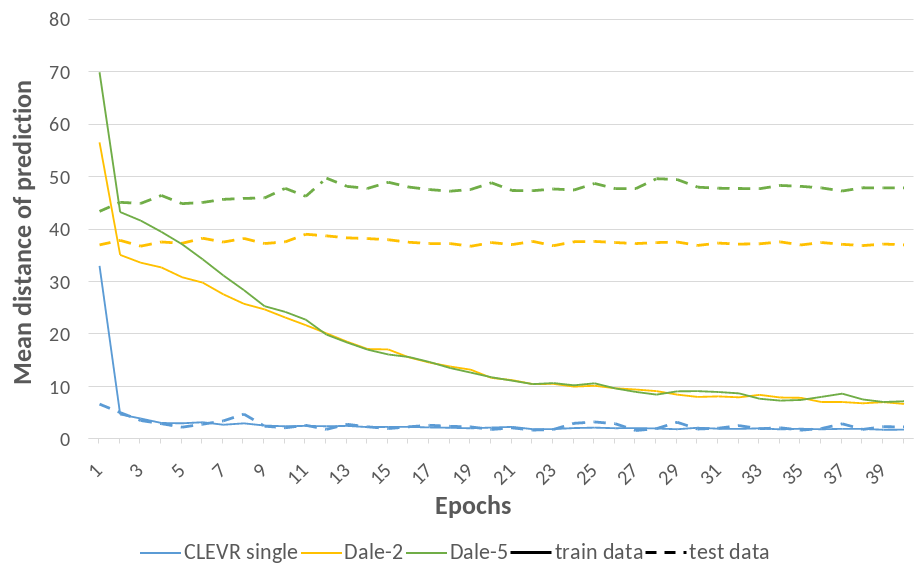
\includegraphics[width=0.8\linewidth]{figures/coordinate-predictor_loss.png}
    \caption{Mean distance between predicted coordinates and ground truth in pixels on different datasets}
    \label{fig:coordinate-predictor_loss}
\end{figure}

Figure \ref{fig:coordinate-predictor_loss} shows the results of the coordinate predictor that doesn't include any information about the target object.
The used feature extractor for these results is \emph{Resnet-3}, but the results don't differ significantly with other feature extractors.
As can be seen, the success between the different datasets differ significantly.
The more objects are present in an image, the worse the model performs.
The model converges for the CLEVR single dataset after around 20 epochs to a mean distance of around 2 pixels.
This prediction even though not perfectly on the center point is always on the object.
Opposed to that, using the Dale-2 dataset with two objects, the mean distance is from the first epoch between 37 and 38 pixels.
With five objects in the Dale-5 dataset, the model only predicts a mean distance of around 45 pixels in the beginning, which worsens with a rising number of epochs to 48 pixels.

An interesting observation is the difference of the mean distances between training and testing data.
The training distance is constantly approaching zero, while the testing loss is staying constant or even getting higher.
This points to the fact that the model is not generalizing the task and learning abstract patterns that can be applied to unseen data, but instead learning the training data by heart.
That is especially visible for the Dale-5 dataset, where learning the patterns of the training data looses even the ability to interpret some patterns in the testing data.
Applying a higher dropout didn't have an impact on the results.

This behavior is indeed not very surprising.
First, these results show that the model is able to derive geometrical information from abstract feature, extracted by a feature extractor.
Geometrical information therefore doesn't get lost during this abstraction, but the model is able to point to a specific object, as long as only one object is part of the image.
Secondly, more than one objects present in an image confuse the model, and it is not able to consistently point to one of them.
This can have multiple reasons, for instance that models lacks the ability to separate objects in the extracted features.
But even given, the model is able to do that and could determine the location of each object in the scene given the feature, it would not be able to tell, which of these is the actual target object.
The guess is then more or less random.
This especially applies to the Dale-2 dataset, where an identification of the target object just based on one distractor is impossible; both of the present objects are unique.
For the Dale-5 dataset, the model could in theory learn that the target object is always the one object which is unique in respect to its and the distractors' attributes.
This task on the other hand seems very difficult to learn.
In conclusion, the models are able to predict geometrical coordinates, but need more information about the target object to identify it.

When the target object \textbf{attributes are encoded as one-hot vectors} and added to the input, the results don't improve.
One factor that now has a much higher impact is the feature extractor that is used.
Table \ref{tab:feature-extractor-mean-distances} compares the mean distances the models predict for the different feature extractors.
The results are shown for the models trained on the Dale-2 and Dale-5 datasets for training and test data.
First, a big difference can be seen between the datasets.
The model only converge to a minimum mean distance of around 46 pixels to the correct coordinates for the Dale-5 dataset, looking at the test data.
In most cases, it stays above 50 pixels.
Using the Dale-2 dataset, the behavior is a little different.
All ResNet extractors with four residual blocks and an additional average pooling and optionally a classifier layers reach similar scores as the experiments before without any one-hot encodings.
Interestingly, without the classifier layer, the model doesn't converge at all and the mean distances jump up and down between the epochs.
This effect also applies when using less residual blocks.
Using the VGG, only VGG-cls2 achieve a similar performance, while the others predict coordinates between 43 and 46 pixels away.

\begin{table}[h]
    \centering
    \begin{tabular}{rcccc}
        \toprule
                            & \multicolumn{2}{c}{\textbf{Dale-2}} & \multicolumn{2}{c}{\textbf{Dale-5}}                                   \\\cmidrule(lr){2-3}\cmidrule(lr){4-5}
                            & train                               & test                                & train          & test           \\\midrule
        \textbf{VGG-0}      & 30,27                               & 46,20                               & \textbf{32,17} & 54,40          \\
        \textbf{VGG-avg}    & \textbf{29,99}                      & 45,08                               & 32,32          & 52,67          \\
        \textbf{VGG-cls1}   & 37,99                               & 43,28                               & 46,57          & 50,75          \\
        \textbf{VGG-cls2}   & 38,87                               & \textbf{39,02}                      & 47,48          & 49,91          \\
        \textbf{VGG-cls3}   & 39,99                               & 44,32                               & 47,26          & \textbf{46,77} \\\midrule
        \textbf{ResNet-3}   & 78,26                               & 65,23                               & 92,07          & 91,12          \\
        \textbf{ResNet-4}   & 44,14                               & 55,24                               & \textbf{36,48} & 58,28          \\
        \textbf{ResNet-avg} & \textbf{33,06}                      & \textbf{39,18}                      & 47,64          & 46,38          \\
        \textbf{ResNet-cls} & 37,57                               & 38,10                               & 44,72          & \textbf{45,92} \\
        \bottomrule
    \end{tabular}
    \caption{Mean test losses for different feature extractors with one-hot attribute encodings after 20 epochs}
    \label{tab:feature-extractor-mean-distances}
\end{table}

Secondly, the training loss now looks also different.
In almost no cases, the models converge to a lower mean distance than with the test data, meaning a higher precision in their predictions, as they did in the experiment before.
The only exception is ResNet-3 as a feature extractor.
In other words, the models are again not able to generalize, but in specific cases memorize the patterns in the train data.
This hints to the fact that only specific layers of the feature extractors contain information that is generally usable to identify and discriminate objects.
Especially the lower layers with fewer residual blocks in the case of ResNet and no classifier layers for the VGG seem to not encode knowledge that can be utilized for this task.
Higher layers, with more specific encoded information need to be used for this research.
The experiments in the following sections are set up using these higher layers.

Adding \textbf{information about the center coordinates} of all objects should have helped the models to get a list of possible predictions.
In theory, the model could learn to choose between these coordinates by relating them to the extracted features of the image.
This hypothesis doesn't hold.
All results for both datasets Dale-2 and Dale-5 are the exact same as without included information about the locations.
The problem therefore doesn't seem to lie in predicting coordinates in general, but predicting the coordinates of the target object.
The model is still not able to understand, which object is the target object.
For that reason, a better representation of the target object is necessary.

In a next step, information about the attributes is included using the \textbf{\emph{GRE-algorithm}} from \citet{Dale1995}.
Again, the mean distance of the predictions as well as the accuracy doesn't improve compared to the previous experiments.

\begin{figure}[h]
    \centering
    \subfigure['Dale-2', train split]{
        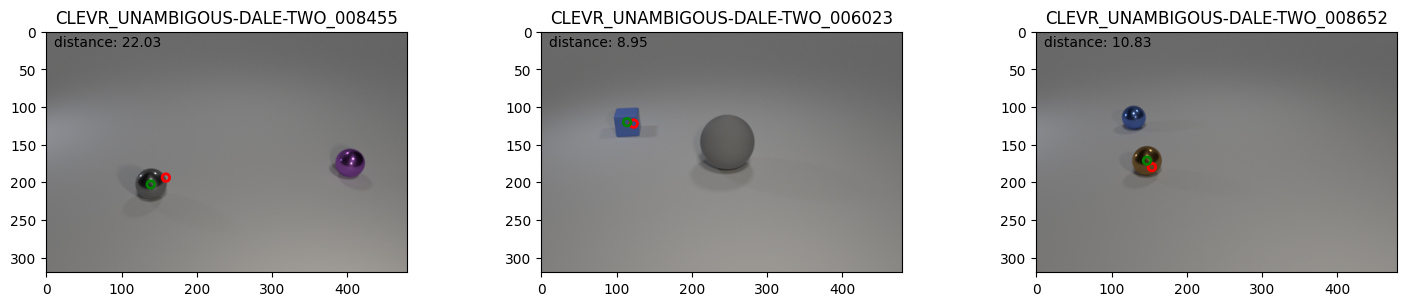
\includegraphics[width=1\linewidth]{figures/visualization_dale-2_train.png}
        \label{fig:visualizations_dale-2_train}
    }
    \subfigure['Dale-2', test split]{
        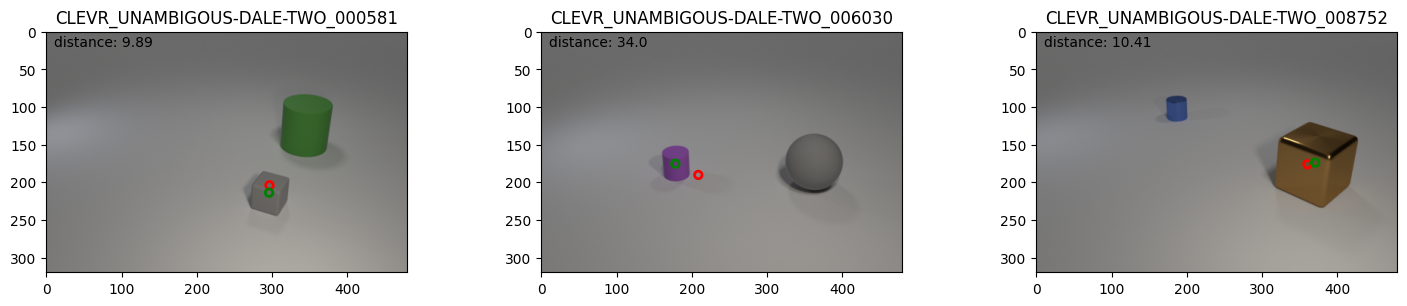
\includegraphics[width=1\linewidth]{figures/visualization_dale-2_test.png}
        \label{fig:visualizations_dale-2_test}
    }
    \subfigure['Dale-5', train split]{
        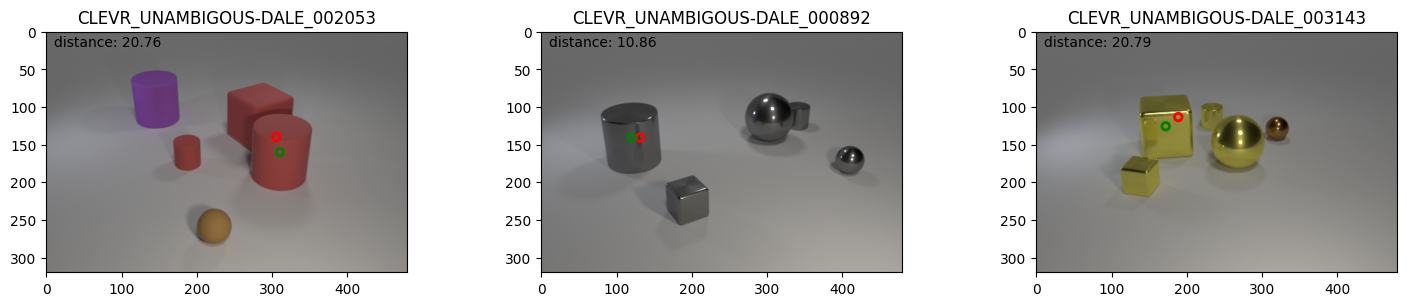
\includegraphics[width=1\linewidth]{figures/visualization_dale-5_train.png}
        \label{fig:visualizations_dale-5_train}
    }
    \subfigure['Dale-5', test split]{
        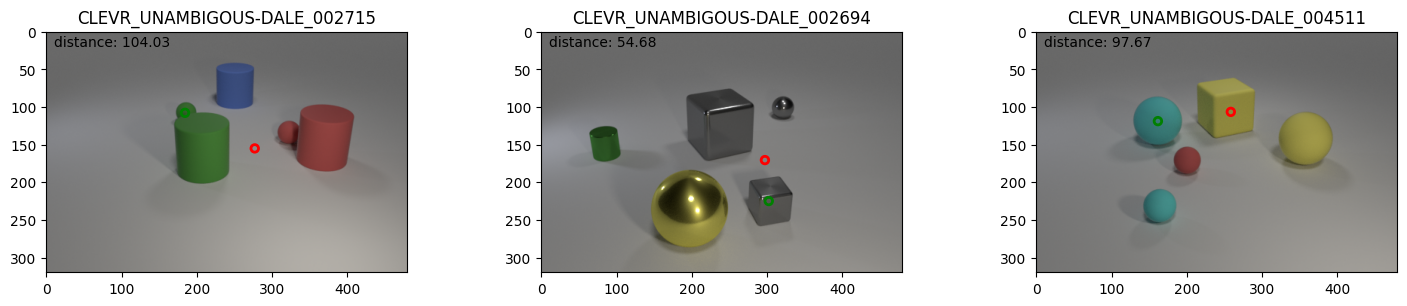
\includegraphics[width=1\linewidth]{figures/visualization_dale-5_test.png}
        \label{fig:visualizations_dale-5_test}
    }
    \caption{Visualization of the models' predictions in the 'Dale' datasets}
    \label{fig:visualizations_dale}
\end{figure}

An interesting pattern appears when doing a qualitative analysis of the models' predictions.
Here, I visualized the predicted coordinates compared to the ground truth coordinates.
Figure \ref{fig:visualizations_dale-2_train} shows random examples of predictions for images in the train dataset of Dale-2.
The green circle shows the ground truth center coordinates of the target object, while the red circle shows the prediction of the model.
As can be seen, the prediction are very precise.
Figure \ref{fig:visualizations_dale-2_complete_train} combines the predictions and ground truths across all images in the train dataset.
Here, all predicted coordinates are placed as red circles into the image, while all ground truth coordinates are places as green circles.
The resulting shape is a rhombus, which reflects that all objects are placed usually central into the scene.
As expected the green and red rhombus align mostly in the same area for the train split of the 'Dale-2' dataset.

The results look very different for the test split.
As can be seen in Figure \ref{fig:visualizations_dale-2_test}, the three randomly selected predictions don't align with the ground truth coordinates.
For all the images, the predictions don't lie on any object.
In the left image as well as in the central image, the predictions are closer to the target object than towards the distractor, but are still quite imprecise.
These findings align with the mean distance scores, described in the sections before.
However, it seems that the model's predictions are all towards the center of the image.
This can be seen clearer in Figure \ref{fig:visualizations_dale-2_complete_test}.
Again, the green circles form the shape of rhombus.
In contrast, the predictions in red almost all cluster in the center of the image.
They form roughly the shape of a smaller rhombus.
This behavior can be observed for all datasets and architectures of the model.
Figures \ref{fig:visualizations_dale-5_train}, \ref{fig:visualizations_dale-5_test}, \ref{fig:visualizations_dale-5_complete_train} and \ref{fig:visualizations_dale-5_complete_test} show the results for the 'Dale-5' dataset.
Here, the model more likely predicts the center coordinates of a distractor object as seen in the right image, which is also reflected in the lower score of the mean distance.
Also the combined visualization shows the same clustering of predictions in the center of the scene, but pattern of the smaller rhombus is better visible.

\begin{figure}[h]
    \centering
    \subfigure['Dale-2', train split]{
        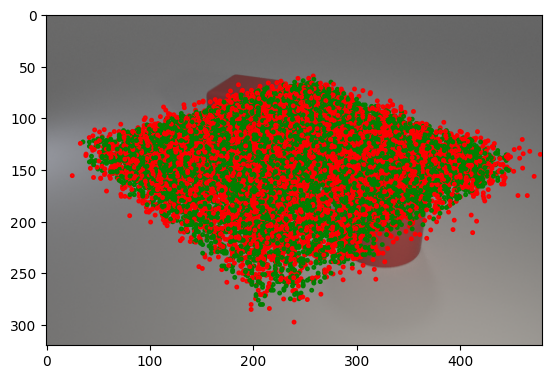
\includegraphics[width=0.42\linewidth]{figures/visualization_dale-2_train_complete.png}
        \label{fig:visualizations_dale-2_complete_train}
    }
    \subfigure['Dale-2', test split]{
        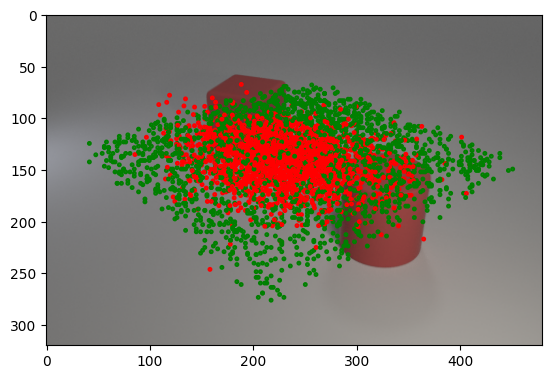
\includegraphics[width=0.42\linewidth]{figures/visualization_dale-2_test_complete.png}
        \label{fig:visualizations_dale-2_complete_test}
    }
    \subfigure['Dale-5', train split]{
        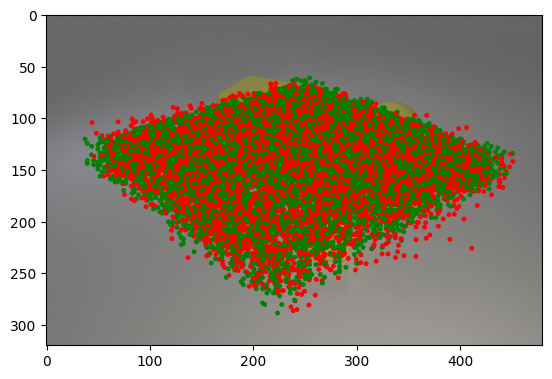
\includegraphics[width=0.42\linewidth]{figures/visualization_dale-5_train_complete.png}
        \label{fig:visualizations_dale-5_complete_train}
    }
    \subfigure['Dale-5', test split]{
        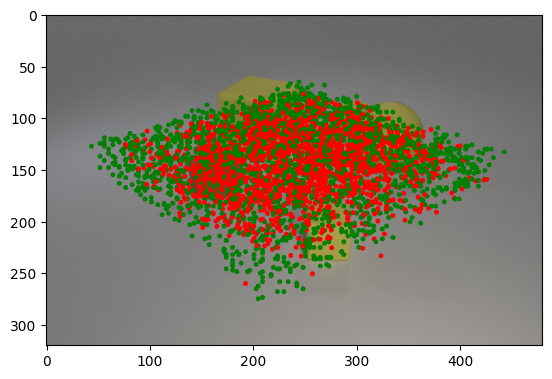
\includegraphics[width=0.42\linewidth]{figures/visualization_dale-5_test_complete.png}
        \label{fig:visualizations_dale-5_complete_test}
    }
    \caption{Visualization of the models' predictions in the Dale datasets}
    \label{fig:visualizations_dale_complete}
\end{figure}

These results allow two conclusions.
First, the models are biased to predict coordinates in the center of the image.
The reason for this is likely that the model can produce a relatively low loss, without relying on many extracted features of the objects.
Since all objects are always located in the center of the image and never in its corners, a prediction of any coordinate in the center is on average closer to the target object than any random prediction or predictions of coordinates at the borders of the image.
The model therefore learns only, where any object is likely located and can minimize the mean distance to a certain extent with this strategy.

Second, even though the models are biased towards the center of the image, the predictions are still often leaning towards the location where many objects lie.
This can be seen for the 'Dale-5' dataset, especially in left and central image in Figure \ref{fig:visualizations_dale-5_test}.
Again, by this strategy, the model can minimize the mean distance, since the probability is high that the target object lies in this cluster of objects.
Concluding, the model is able to extract, where objects are located in the image, but can't decide, which of these objects is the target object.

\subsubsection{Bounding Box classifier}

\subsubsection{Caption generator}
In the next paragraphs, the results of the caption generator will be discussed.
Table \ref{tab:results_caption-generator} shows the different scores of the models, when trained on 'Dale-2' and 'Dale-5'.
ResNet-3 produced the best results, when it was used as a feature extractor.
The results are shown after 50 epochs, but the scores already start to converge after 20 epochs and changed only very in the following epochs.

\begin{table}[h]
    \centering
    \begin{tabular}{rccc}
        \toprule
                               & \textbf{Accuracy} & \textbf{Word-by-word accuracy} & \textbf{Non-target accuracy} \\
        \textbf{Dale-2}        & 49\%              & 82\%                           & 48\%                         \\
        \textbf{Dale-2 masked} & 72\%              & 90\%                           & 25\%                         \\
        \textbf{Dale-5}        & 21\%              & 45\%                           & 40\%                         \\
        \textbf{Dale-5 masked} & 21\%              & 54\%                           & 45\%                         \\
        \bottomrule
    \end{tabular}
    \caption{Results of the caption generator, based on ResNet-3}
    \label{tab:results_caption-generator}
\end{table}

The sum of the \emph{accuracy} and the \emph{non-target-accuracy} adds to 97\%, when trained on the 'Dale-2' dataset.
This means that the models produce almost always correct descriptions of an object in the image.
Moreover, these descriptions are also efficient in the way that they follow the GRE-algorithm of \citet{Dale1995} and only use necessary discriminative attributes.
Features of both objects are therefore extracted perfectly and related to the vocabulary.
As expected, the model has difficulties to decide, which of both objects is the target object, since no information is passed to the model.
With 48\% of the images describing the target object and 49\% of the images describing the distractor, the model uses a random guess.
This changes, when also the masked image is presented to the model.
Then, the accuracy for the target object is with 72\% well above chance.
Still, the wrong descriptions describe almost every time the distractor object.
This indicates that the problem doesn't lie in extracting features of objects, but only in deciding which object in the image to describe.

When the model is trained on the 'Dale-5' dataset, the results are much worse.
Now, without masking only in 61\% of the images, the model describes any of the objects in the image.
With 21\% of these descriptions being a description of the target object, the model again uses a random guess.
Interestingly, passing the masked image to the model doesn't help it to identify the correct object.
The accuracy stays at the same value.
In contrast, the non-target accuracy is increased by 5\% points.
The model is more likely to identify a wrong object.
Furthermore, the word-by-word accuracy increases from 45\% to 54\%.
This increase is likely due to the fact that the description of the target object often shares some attributes with distractor objects.
For instance an image with a target object being a \emph{small red cube} was identified as a \emph{<pad> <pad> cube} when the model didn't receive the masked image.
After also the masked image was passed to the model, it generated the description \emph{small blue cube}.
This was the correct description of a distractor and because of the overlap of the attributes, the word-by-word accuracy increased from 33\% to 66\%.

The approach, how the padding is produced and in which order the attributes are concatenated didn't have an effect on the described metrics.
When the order was reversed and the padding appended, it seemed like the model was converging slightly faster and reaching the limit around tow to three epochs earlier.
The final peak stayed exactly the same and the effect was therefore not studied deeper if there is an actual significant difference.

There are two main possible explanations for the big difference between the two datasets.
First, as already seen in the experiments before, the bigger number of distractors confuses the model more, where to focus on.
In the 'Dale-2' dataset, there are only two possibilities, while the four distractors in the 'Dale-5' dataset give the model a bigger choice.
The second explanation lies in the used GRE-algorithm.
When only two random objects are placed in a scene, the probability that only the shape is enough to discriminate the objects is at 66,6\%, namely the caption is only one word long.
For shape and color, the probability lies at 29,2\% and that all three attributes are necessary is 4,1\%.
Opposed to that the probabilities with four distractors are 19,8\%, 47\% and 33,2\% respectively.
With four distractors the algorithm is much more likely to produce longer captions.
These are harder to generate for the model, since it needs to take more attributes into account to discriminate the target object from the distractors.

\subsection{Language games}
\subsubsection{Discrimination games}
There are five variables in the experiments that are adjusted:
(1) the image embedding size for the sender $e_s$, (2) the LSTM hidden size for the sender $h_s$, (3) the image/message embedding size for the receiver $e_r$, (4) the LSTM hidden size for the receiver $h_r$ and (5) the size of the vocabulary $|V|$.

Table \ref{tab:results_discriminator} shows the accuracy of the models calculated on the success of communication if the receiver can identify the target object.
A random guess corresponds to 50\% in the \emph{Dale-2} dataset and 20\% in the \emph{Dale-5} dataset.
Four different vocabulary sizes $|V|$ are tested.
A size of 13 symbols corresponds to the 13 attributes the objects can have and align with human language.
If the symbols were similarly used, messages would have lengths between one and three symbols.
Opposed to that a slightly smaller vocabulary with 10 symbols is used to create a smaller bottleneck with a higher pressure to condense the information.
Similarly, a bigger vocabulary consisting of 20 symbols tests how a bigger bottleneck changes the results.
Lastly, a big vocabulary of 100 symbols should give the model all options to encode the information, including one symbol per attribute or one symbol describing a combination of attributes.

The hidden sizes $h_s$ and $h_r$ as well as the embedding sizes $e_s$ and $e_r$ are chosen in alignment with the vocabulary size.
The hidden sizes are always smaller or equal to the vocabulary size since the information about each word needs to be compressed in a smaller dimension to learn meaning.
Hereby, hidden sizes of 10 and 100 are tested.
On the other hand, three different embedding sizes are tested: 10, 50 and 100.
The reason for this is to experiment, what is the optimal middle ground between compressing features of an image encoded in high dimension vectors and upscaling encoded messages in low dimension vectors.

\begin{table}[h]
    \centering
    \begin{tabular}{ccccc|cc|cc|cc}
        \toprule
              &         &         &         &         & \multicolumn{2}{c}{\textbf{Dale-2}} & \multicolumn{2}{c}{\textbf{Dale-5}} & \multicolumn{2}{c}{\textbf{CLEVR color}}                                                         \\\cmidrule(lr){6-7}\cmidrule(lr){8-9}\cmidrule(lr){10-11}
        $|V|$ & $h_{s}$ & $h_{r}$ & $e_{s}$ & $e_{r}$ & \textbf{Accuracy}                   & \textbf{length}                     & \textbf{Accuracy}                        & \textbf{length} & \textbf{Accuracy} & \textbf{length} \\\midrule
        {10}  & {10}    & {10}    & {10}    & {10}    & {96,4\%}                            & {1,99}                              & {24,7\%}                                 & {1}             & {17,3\%}          & {2}             \\
        {10}  & {50}    & {50}    & {50}    & {50}    & {50\%}                              & {2}                                 & {21,4\%}                                 & {2}             & {17,8\%}          & {1}             \\
        {13}  & {10}    & {10}    & {10}    & {10}    & {94,9\%}                            & {2}                                 & {24,8\%}                                 & {2}             & {17,1\%}          & {2}             \\
        {13}  & {10}    & {10}    & {50}    & {50}    & {49,6\%}                            & {2}                                 & {21,9\%}                                 & {2}             & {17,9\%}          & {1}             \\
        {20}  & {10}    & {10}    & {50}    & {50}    & {50,9\%}                            & {1}                                 & {23\%}                                   & {2}             & {15,9\%}          & {2}             \\
        {100} & {10}    & {10}    & {10}    & {10}    & {97,3\%}                            & {2}                                 & {24\%}                                   & {2}             & {18,1\%}          & {2}             \\
        {100} & {10}    & {10}    & {50}    & {50}    & {49,9\%}                            & {2}                                 & {24,4\%}                                 & {2}             & {15,8\%}          & {2}             \\
        {100} & {100}   & {100}   & {100}   & {100}   & {49\%}                              & {1}                                 & {25,3\%}                                 & {2}             & {15,6\%}          & {1}             \\
        \bottomrule
    \end{tabular}
    \caption{Results of the discriminators: $|V|$ are different vocabulary sizes, $h$ hidden sizes and $e$ embedding sizes.}
    \label{tab:results_discriminator}
\end{table}

For the \emph{Dale-2}, a clear correlation between the hidden sizes, embedding sizes and the size of the vocabulary can be identified.
A hidden/embedding size as high as the vocabulary size is beneficial for identifying the correct object.
The receiver identifies almost every sample correctly when all sizes are 10.
When the hidden and embedding sizes are increased, the guesses by the receiver are random with 50\% accuracy.
Interestingly, a vocabulary size of 10 is enough to communicate a meaningful message when the model is trained on the \emph{Dale-2} dataset.

The results change, when using the \emph{Dale-5} dataset with four distractors.
With four distractors and with low hidden, embedding and vocabulary sizes, the agents barely pass the random baseline with 23\%.
Only increasing the vocabulary size to 100 raises the accuracy by almost 20\% points to 43\%.
This is still considerably lower than the 95\% of the \emph{Dale-2} dataset.
The same applies to the 'CLEVR color' dataset, where all models achieve a very low accuracy of around 15 to 17\%, corresponding to random guesses.

\cmtDK{calculation of loss?}
\cmtDK{length}

Two conclusions can be drawn.
First, the hidden as well as the embedding sizes need to be close to the vocabulary size.
This even applies for very low vocabulary sizes, which means that the image encodings need to be compressed to the same low dimensions.
The reason for this is very likely that neural models have difficulties to upscale from lower dimensions (e.g. from low $h_r$ to high $e_r$) as opposed to learn how to extract the important information from a vector with many dimensions.

The second conclusion that can be drawn looks at the differences between the two datasets.
Unsurprisingly, the agents have a much higher difficulty to discriminate a target object from four instead of one distractor.
Since we discriminate objects based on properties that are also distinguished in human cognition (color, size, shape), we expect that the vocabulary onto which the agents converge reflects these categories and is therefore close to human vocabulary.
There are 48 possible combinations of attributes.
Still, for Dale-2, a vocabulary size of only 10 is enough for an almost perfect accuracy with two objects.
This hints to the fact that the agents don't describe the complete target object, but only rely on discriminative attributes between the objects.
The need for a more detailed description of discriminative attributes is higher when more distractors are involved.
Therefore, the models need to learn more combinations of symbols in order to attest to this higher level of detail and especially how to relate them to features in the images.

\cmtDK{look at language}
\cmtDK{similarity to bounding box classifier}

\subsubsection{Caption generators}
\begin{table}[h]
    \centering
    \begin{tabular}{ccc|ccc|ccc}
        \toprule
              &         &         & \multicolumn{3}{c}{\textbf{Dale-2}} & \multicolumn{3}{c}{\textbf{Dale-5}}                                                                             \\\cmidrule(lr){4-6}\cmidrule(lr){7-9}
        $|V|$ & $h_{s}$ & $h_{r}$ & \textbf{Acc.}                       & \textbf{word-by-word}               & \textbf{length} & \textbf{Acc.} & \textbf{word-by-word} & \textbf{length} \\\midrule
        {10}  & {10}    & {10}    & {22,9\%}                            & {62,8\%}                            & {2}             & {7,1\%}       & {40\%}                & {2}             \\
        {13}  & {10}    & {10}    & {22,8\%}                            & {62,9\%}                            & {1}             & {7,3\%}       & {38,7\%}              & {2}             \\
        {20}  & {10}    & {10}    & {24,6\%}                            & {64\%}                              & {2}             & {6,7\%}       & {38,7\%}              & {2}             \\
        {100} & {10}    & {10}    & {24,4\%}                            & {62\%}                              & {2}             & {7,8\%}       & {40\%}                & {2}             \\
        {100} & {100}   & {100}   & {21\%}                              & {62\%}                              & {2}             & {6,5\%}       & {37,8\%}              & {2}             \\
        \bottomrule
    \end{tabular}
    \caption{Results of the caption generator: $|V|$ are different vocabulary sizes and $h$ hidden sizes.}
    \label{tab:results_caption_generator_game}
\end{table}

The results of the caption generator game are summarized in Table \ref{tab:results_caption_generator_game}.
In general, it can be seen that the agents have much bigger problems, to solve the task together than a single neural network.
The highest accuracy for descriptions, the agents manage to predict correctly is at 24,6\% for images of the 'Dale-2' dataset.
Compared to the (masked) accuracy of the single model with 72\%, the agents predict 47,4\% points less correct descriptions.
A similar worse performance can be seen for the 'Dale-5' dataset.
Here, the agents only manage to produce for 7,8\% of the images correct descriptions, 13,2\% points less than the single neural model.
The same effect can be seen for the word-by-word accuracy, which is much lower than the metric for the single neural model for both datasets.

When looking, how the different variables affect the performance, it can be seen that a bigger vocabulary size tends to help the agents.
This is only visible for the 'Dale-2' dataset.
With constant hidden sizes of 10, the agents score around 22,9\% with only 10 and 13 available symbols.
When this is increased to 20 and respectively 100 symbols, the agents can increase their accuracy to around 24,5\%.
However, the increase is relatively small.
Interestingly, this effect only occurs, when the hidden sizes are small with only 10 dimensions.
As soon as they are increased to 100 dimensions with a vocabulary size of 100 symbols, the accuracy drops to 21\%.

Looking at the 'Dale-5' dataset, the increase is still there, when the vocabulary is increased to 100 symbols.
Nonetheless, the difference is with 0,5\% points even smaller and the reason may be due to other influences, such as the random initialization of the weights of the agents.
This would need to be confirmed in future experiments.

An interesting observation can be made about the length of the messages, the sender generates.
In almost all cases, the average length is 2 symbols.
Only in one configuration, the sender produces single symbol messages.
This happens, when the vocabulary size is 13, the same number as possible features the objects can have.
In this case, the accuracy, as well as the word-by-word accuracy stay the same compared to the configuration with a vocabulary of only 10 symbols.

\cmtDK{look at language more detailed}

\subsubsection{Coordinate predictors}
In the final setup, the agents are tasked with communicating objects with fewer infused human knowledge.
Table \ref{tab:results_dale_predictor_game} shows the results for the setup, in which the sender is pointed towards the target object with a human description based on the GRE algorithm.
Hereby, the 'CLEVR single' dataset acts as a baseline, to test if the agents are able to predict coordinates of objects at all.
In every configuration of the variables, the agents achieve a very high performance.
The worst average distance across the test dataset is 10 pixels, which still points on an object.
Also the accuracy, which evaluates how many guesses of the receiver were pointing on an object reflects this fact.
All configuration achieve an accuracy higher than 96,7\%.
This aligns also with the results from the single neural models, where the average distance was similarly low.
In general, this shows that the agents are able to predict coordinates together.
However, the question arises if the message by the sender has actually an effect on the receivers' decision, or if the receiver learns to point towards the target coordinates on his own and the message is ignored.
When a different sender is used that is receiving the masked image as input, the results indicate that the message has in fact an influence and the receiver learns how to interpret the message.
The results for this setup are summarized in \ref{tab:results_masked_predictor_game}.
In three of six experiments, the agents predict much higher average distances.
In one case, the mean distance lies at 19,8 pixels, while the accuracy is only at 55,1\%.
Since the receiver is the same in both setups, this observation indicates that a meaningful message is communicated between the agents.

\begin{table}[h]
    \centering
    \begin{tabular}{ccc|ccc|ccc|ccc}
        \toprule
              &         &         & \multicolumn{3}{c}{\textbf{CLEVR single}} & \multicolumn{3}{c}{\textbf{Dale-2}} & \multicolumn{3}{c}{\textbf{Dale-5}}                                                                                                       \\\cmidrule(lr){4-6}\cmidrule(lr){7-9}\cmidrule(lr){10-12}
        $|V|$ & $h_{s}$ & $h_{r}$ & \textbf{Dist.}                            & \textbf{Acc.}                       & \textbf{length}                     & \textbf{Dist.} & \textbf{Acc.} & \textbf{length} & \textbf{Dist.} & \textbf{Acc.} & \textbf{length} \\\midrule
        {10}  & {10}    & {10}    & {10,1}                                    & {98,5\%}                            & {2}                                 & {36,5}         & {19,9\%}      & {2}             & {45,7}         & {14,4\%}      & {2}             \\
        {13}  & {10}    & {10}    & {6}                                       & {99\%}                              & {1}                                 & {38}           & {20,4\%}      & {2}             & {47,3}         & {10,8\%}      & {2}             \\
        {20}  & {10}    & {10}    & {9,7}                                     & {96,7\%}                            & {2}                                 & {37,3}         & {21,2\%}      & {2}             & {47,3}         & {11,3\%}      & {1}             \\
        {100} & {10}    & {10}    & {7,7}                                     & {98,4\%}                            & {2}                                 & {40,4}         & {21,7\%}      & {2}             & {45,4}         & {10,8\%}      & {2}             \\
        {100} & {100}   & {100}   & {7,5}                                     & {96,9\%}                            & {2}                                 & {40,1}         & {17,8\%}      & {2}             & {44,3}         & {11,8\%}      & {1}             \\
        \bottomrule
    \end{tabular}
    \caption{Results of the description coordinate predictor: $|V|$ are different vocabulary sizes and $h$ hidden sizes.}
    \label{tab:results_dale_predictor_game}
\end{table}

When the experiments are run, using the 'Dale-2' dataset, the results are much worse.
For the \emph{description coordinate predictor}, the average distance ranges from 36,5 pixels to 40,4 pixels.
The configuration with a vocabulary size of only 10 symbols fares the best, while a vocabulary of 100 symbols produces the worst results.
Still, the accuracy shows that around 19,9\% to 21,7\% of the guesses are on the target object.
Here, the configurations with higher vocabulary sizes fare better, even though the differences are very small and may be due to other factors.
Interestingly, when comparing the two configurations with a vocabulary size of 100 symbols one can see that the average distance is similar, but the accuracy is significantly higher when the hidden sizes are lower.
In other words, with lower hidden sizes the agents can make more correct guesses.
Overall, it can be seen that a higher vocabulary size lets the agents' guesses get in general closer to the target object, but they are less precise on the object itself.

The results for 'Dale-5' dataset are even worse, but are comparable with the results with a single neural model.
Apparently, the agents are not able to communicate the target object, and the predictions by the receiver are general in the middle of the image, which results in an average distance of around 45 to 50 pixels.
The differences of the mean distances are not very significant in this range, to allow an analysis of the different configurations.
The only metric that stands out is the accuracy of the configuration with a vocabulary size of 10 symbols.
With 14,4\%, it is 2,6\% points higher than the next best accuracy.
It is able to predict the center coordinates of the target object the most precise.

\begin{table}[h]
    \centering
    \begin{tabular}{cccc|ccc|ccc|ccc}
        \toprule
              &         &          &         & \multicolumn{3}{c}{\textbf{CLEVR single}} & \multicolumn{3}{c}{\textbf{Dale-2}} & \multicolumn{3}{c}{\textbf{Dale-5}}                                                                                                       \\\cmidrule(lr){5-7}\cmidrule(lr){8-10}\cmidrule(lr){11-13}
        $|V|$ & $h_{s}$ & $h_{r}$  & $e_{s}$ & \textbf{Dist.}                            & \textbf{Acc.}                       & \textbf{length}                     & \textbf{Dist.} & \textbf{Acc.} & \textbf{length} & \textbf{Dist.} & \textbf{Acc.} & \textbf{length} \\\midrule
        {10}  & {10}    & {10}     & {1024}  & {19,8}                                    & {55,1\%}                            & {2}                                 & {34,8}         & {24,3\%}      & {1}             & {44,3}         & {11,8\%}      & {2}             \\
        {10}  & {10}    & {10}     & {512}   & {9,3}                                     & {92\%}                              & {2}                                 & {36,3}         & {19,9\%}      & {1
        ,7}   & {45,9}  & {12,7\%} & {2}                                                                                                                                                                                                                                   \\
        {13}  & {10}    & {10}     & {1024}  & {7,8}                                     & {96,8\%}                            & {2}                                 & {36,3}         & {20,2\%}      & {1}             & {45,4}         & {11,4\%}      & {2}             \\
        {20}  & {10}    & {10}     & {1024}  & {6,6}                                     & {98,3\%}                            & {2}                                 & {37,8}         & {16,1\%}      & {2}             & {45,2}         & {11\%}        & {2}             \\
        {100} & {10}    & {10}     & {1024}  & {5,2}                                     & {98,5\%}                            & {2}                                 & {37,4}         & {20,1\%}      & {2}             & {43,6}         & {16,7\%}      & {2}             \\
        {100} & {100}   & {100}    & {1024}  & {12,5}                                    & {92,1\%}                            & {2}                                 & {36,5}         & {20,7\%}      & {2}             & {44,6}         & {12,7\%}      & {2}             \\
        \bottomrule
    \end{tabular}
    \caption{Results of the masked coordinate predictor: $|V|$ are different vocabulary sizes, $h$ hidden sizes and $e$ embedding sizes.}
    \label{tab:results_masked_predictor_game}
\end{table}

Finally looking at the
